\section{System Model}\label{sec:model}
Table~\ref{tab:notation} lists the main symbols. Assumptions used only in the analysis are numbered.

\begin{table}[t]\centering
\caption{Main notation}\label{tab:notation}
\footnotesize
\begin{tabular}{@{}ll@{}}
\toprule
Symbol & Meaning\\
\midrule
$G=(\mathcal C,\mathcal E)$ & cell graph; $\mathcal E$: pairs of adjacent cells (gateway pairs)\\
$\mathcal M$ & media: every cell and every gateway pair\\
$V$, $V_{\mathrm p}\subseteq V$ & devices; devices eligible as AI nodes\\
$K\subseteq\mathcal C$ & critical cells, i.e., cells hosting an AI node\\
$Q$, $\Tp$ & packets of the query; airtime of one UAV packet\\
$\tau_f$ & medium occupancy of one acknowledged ground hop\\
$q(t)$, $T_{\mathrm f}$ & track of team~1; flight duration\\
$P_c(x)$ & probability that cell $c$ hears a packet sent above $x$\\
$C_k$ & completion time of critical cell $k$\\
$E_u$ & energy budget of device $u$ for one mission\\
$\pi_c$ & prior probability that the person is in cell $c$\\
$c^\star$, $\omega$ & cell of the person; all other randomness\\
$T^\star$ & time from take-off until the person is confirmed\\
\bottomrule
\end{tabular}
\end{table}

\subsection{Area and terrain}
We surveyed $10\times10$\,km windows of eight protected areas with OpenStreetMap and a 25\,m elevation grid
(Table~\ref{tab:terrain}). They fall into two groups. In lowland or gently rolling forest the elevation varies by less
than 50\,m within 100\,m of a cell centre, small against the flight altitude of 100\,m. In mountain parks it varies by
90--160\,m (median) and up to 300\,m (90th percentile), more than the flight altitude, and more than half of the area
can be steeper than $30^\circ$. Our model treats the ground as a plane and therefore covers the first group; the second
needs terrain-following flight and terrain shadowing of both A2G and ground links.

\begin{assumption}[Flat ground]\label{as:flat}
Devices lie on a plane; the UAV flies at constant height $h$ above it.
\end{assumption}

\begin{table}[t]\centering
\caption{Terrain of four of the eight surveyed $10\times10$\,km windows}\label{tab:terrain}
\footnotesize
\begin{tabular}{@{}lrrrr@{}}
\toprule
Window & Elev.\ (m) & Slope & $>30^\circ$ & Relief (m)\\
\midrule
Cat Tien (VN) & 83--247 & $4^\circ$ & 0\,\% & 14 / 26\\
Bayerischer Wald (DE) & 764--1\,440 & $10^\circ$ & 0\,\% & 44 / 79\\
Bach Ma (VN) & 32--1\,455 & $28^\circ$ & 40\,\% & 126 / 185\\
Hoang Lien (VN) & 1\,180--3\,117 & $32^\circ$ & 58\,\% & 156 / 227\\
\bottomrule
\multicolumn{5}{@{}p{0.95\columnwidth}@{}}{\scriptsize Slope: median. $>30^\circ$: share of the area steeper than
$30^\circ$. Relief: elevation range within 100\,m of a cell centre, median / 90th percentile over the cells. The other
four windows (Cuc Phuong, Yosemite, Great Smoky Mountains, Kinabalu) belong to the mountain group.}
\end{tabular}
\end{table}

\subsection{Network, cells and devices}
The area is tiled by hexagonal cells of radius $R_{\mathrm c}=100$\,m. Every cell has a cell leader (CL); two adjacent
cells are joined by exactly one gateway pair; cell channels follow a 7-colour reuse and every gateway pair has its own
radio and channel. Let $G=(\mathcal C,\mathcal E)$ be the cell graph. Cells are grouped into clusters of at most 80
cells, each with a cluster head (CH) that has a LoRa uplink to the BS. Every cell and every gateway pair is one
\emph{medium} $m\in\mathcal M$: at most one of its radios transmits at a time.

The devices $V$ are camera traps, acoustic and wildfire sensors. A subset $V_{\mathrm p}\subseteq V$ can serve as AI
nodes: devices in a clearing with a solar panel and a neural accelerator, or an edge box next to them. A cell that hosts
an AI node is a \emph{critical cell}; $K$ denotes their set. Cells without devices (rivers, swamps) are holes of $G$.

\textbf{Density.} The cell graph is connected only if every cell has devices close enough to its neighbours. With an
urban street-canyon model of the ground links this requires devices at most about 50--60\,m apart, i.e., roughly 300
devices per km$^2$ \todo{redo for the foliage model of Section~\ref{sec:g2g}}. We use 816 devices per km$^2$ as in our
conference version. Real forest deployments are far sparser (Fig.~\ref{fig:density}): park-wide densities range from
0.003 to 2 devices per km$^2$, and only small pilot sites exceed 100. These sparse networks connect devices directly to
4G, LoRa or satellites, or not at all. Our density is therefore a forward-looking assumption, motivated by falling device
prices, by vendors that already deploy tens of thousands of forest sensors \cite{dryad}, and by the possibility of
sharing one mesh among camera, fire and acoustic networks. Section~\ref{sec:eval} reports the sensitivity to lower
densities. \todo{sensitivity to 400 and 280 devices per km$^2$.}

\begin{figure}[t]\centering
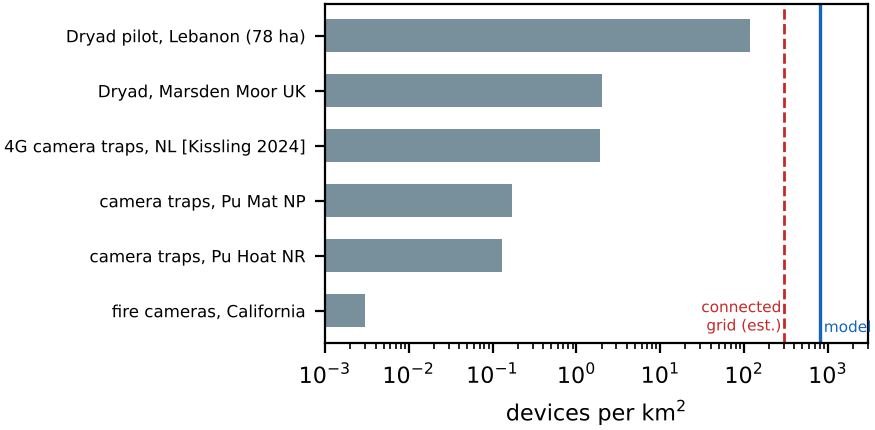
\includegraphics[width=\columnwidth]{draft2-density-gap-labelled.png}
\caption{Device density of real forest deployments (bars, log scale) against the density at which a cell grid of radius
100\,m stays connected (dashed, urban estimate) and the density of our model (solid). Densities are devices divided by
the area stated in each source.}\label{fig:density}
\end{figure}

\subsection{Energy and wake-up}\label{sec:energy}
All devices run on batteries, possibly with a small solar panel that is weak under the canopy. A device sleeps between
its own sensing events. Device $u$ has an energy budget $E_u$ for one mission; it spends $e_{\mathrm{rx}}$ per second
awake with its radio listening and $e_{\mathrm{tx}}$ per transmitted frame. When a mission starts, the BS broadcasts a
LoRa message with the mission identifier and the take-off time; from the plan, the devices of cell $c$ compute a wake
window $[t^{\mathrm{on}}_c,t^{\mathrm{off}}_c]$ that covers the UAV pass over $c$ and the ground transport through $c$.
\open{energy numbers of a camera trap and a sensor node; whether the CH stays awake.}

\subsection{UAVs and emission}
Team~1 is a fixed-wing VTOL at height $h=100$\,m with speed $v\in[25,50]$\,m/s and bank angle at most $45^\circ$, hence a
turning radius $\rho(v)=v^2/g$: 255\,m at 50\,m/s and 63.7\,m at 25\,m/s. It broadcasts one packet of 99\,B payload every
$\Tp=10$\,ms. Its track is a curve $q:[0,T_{\mathrm f}]\to\mathbb R^2$ from and to the BS; packet $s$ is emitted at
$q(t_s)$. Team~2 is a rotary-wing UAV flying at 15\,m/s; verifying one cell takes $\sigma\approx78$\,s.

\subsection{Air-to-ground reception through the canopy}
At slant distance $\ell=\sqrt{d^2+h^2}$ the path loss is free space up to $d_0=100$\,m ($PL_0=80.05$\,dB at 2.4\,GHz)
and grows with exponent $\alpha=3$ beyond, plus an excess loss $L_{\mathrm{obs}}$ due to the foliage:
\begin{equation}
PL(\ell)=PL_0+10\alpha\log_{10}(\ell/d_0)+L_{\mathrm{obs}},\qquad \ell\ge d_0 .\label{eq:pl}
\end{equation}
Each packet sees independent Rician fading with $K=2$ and is received when the faded power exceeds an effective
threshold $S$. With transmit power $P_{\mathrm t}=10$\,dBm, a device at horizontal distance $d$ receives a packet with
probability
\begin{equation}
p(d)=\Pr\bigl\{g>10^{(S-P_{\mathrm t}+PL(\ell))/10}\bigr\},\quad 2(K{+}1)g\sim\chi'^2_2(2K).\label{eq:pd}
\end{equation}
We summarise a regime by $R_{50}$, the horizontal distance at which $p=1/2$. The four regimes $L_{\mathrm{obs}}=0$, 9.0,
19.8 and 25.7\,dB give $R_{50}=1016$, 498, 199 and 99\,m; $S=-101.04$\,dBm reproduces the reception measured in ns-3 in
all four with a root-mean-square error of at most 0.003.

The regimes map onto foliage depth. Weissberger's model \cite{weissberger1982} gives the loss of a path through $x$
metres of trees as $0.45f^{0.284}x$\,dB for $x\le14$\,m and $1.33f^{0.284}x^{0.588}$\,dB for $14<x\le400$\,m, with $f$ in
GHz. At 2.4\,GHz, 9, 20 and 26\,dB correspond to 17, 66 and 103\,m of trees on a horizontal path. A slant path at
elevation angle $\theta$ crosses a canopy layer of depth $h_{\mathrm c}$ over $h_{\mathrm c}/\sin\theta$ metres; for
$h_{\mathrm c}=10$\,m this gives 8\,dB at $45^\circ$ and 17.5\,dB at $11^\circ$ (Fig.~\ref{fig:canopy}). A constant
$L_{\mathrm{obs}}$ is thus an approximation of a loss that grows with distance, and Weissberger's model was fitted on
horizontal paths, so its use for slant paths is an extrapolation. \todo{angle-dependent variant
$L_{\mathrm{obs}}(\theta)$ as sensitivity; calibrate on the UAV 802.15.4 dataset of \cite{nekrasov2019}.}

\begin{figure}[t]\centering
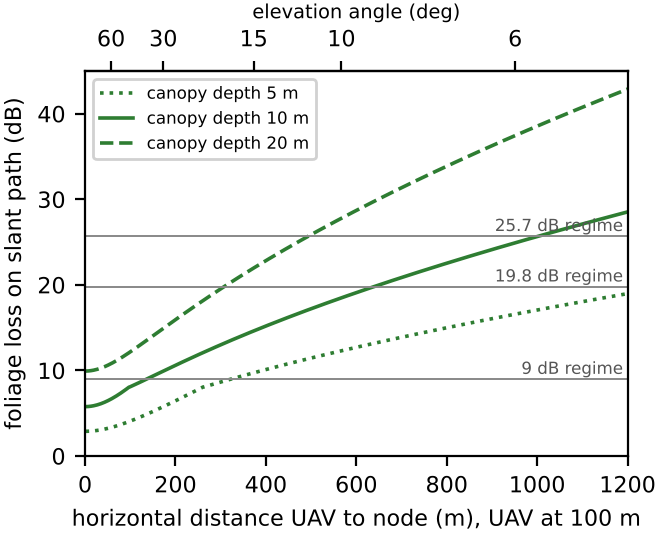
\includegraphics[width=0.92\columnwidth]{draft2-canopy-loss-labelled.png}
\caption{Weissberger foliage loss on the slant path from a UAV at 100\,m to a device under a canopy of depth 5, 10 and
20\,m, versus horizontal distance (bottom) and elevation angle (top). Horizontal lines: the constant excess losses of
the three canopy regimes.}\label{fig:canopy}
\end{figure}

\begin{figure}[t]\centering
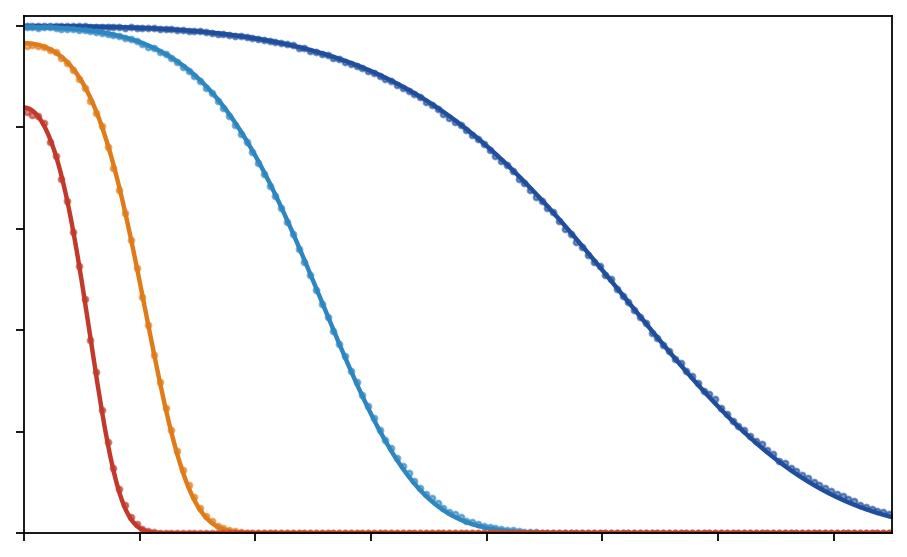
\includegraphics[width=0.86\columnwidth]{nd1-channel-p-of-d-model-vs-ns3.png}
\caption{Packet reception versus horizontal distance for the four regimes, from $R_{50}=1016$\,m (rightmost) to 99\,m.
Dots: ns-3 passes in 10\,m bins. Lines: model \eqref{eq:pd} with one common threshold. \todo{labelled version.}}
\label{fig:channel}
\end{figure}

The CL gathers what the devices of its cell hold, so the relevant event is that some device of the cell hears the
packet. For a cell $c$ with device set $U_c$ and the UAV above $x$,
\begin{equation}
P_c(x)=1-\prod_{u\in U_c}\bigl(1-p(\lVert x-u\rVert)\bigr).\label{eq:pcell}
\end{equation}
\begin{assumption}[Independent receptions]\label{as:indep}
Receptions of one packet at different devices are independent.
\end{assumption}
Assumption~\ref{as:indep} is used only in \eqref{eq:pcell}; the bounds of Section~\ref{sec:limits} need only the
marginals $P_c(x)$.

\subsection{Ground links under the canopy}\label{sec:g2g}
Ground links follow a log-distance model with exponent 3.5, log-normal shadowing ($\sigma=7.8$\,dB, drawn once per
device pair) and Rayleigh fading in 100\,ms blocks, plus a foliage excess loss $L_{\mathrm f}(d)$ for a link of length
$d$. With Weissberger's model, $L_{\mathrm f}$ is 12.6\,dB at 30\,m, 17\,dB at 50\,m and 25.6\,dB at 100\,m.
\open{a model measured for devices near the ground in forest; the exponent 3.5 and the shadowing come from an urban
street model \cite{tr38901} and the two losses may double count.} Under CSMA/CA with acknowledgements, an acknowledged hop
of a 127\,B frame occupies its medium for at least 4.8\,ms and for $\tau_f\approx5$--7\,ms in practice.

\subsection{Query, coding and completion}
The query consists of $L=12$ reference images, $Q=4041$ packets in total. The UAV repeats the query along its track;
with a rateless code a cell decodes once it holds $\lceil(1+\epsilon)Q\rceil$ distinct coded packets ($\epsilon=0.05$),
and no code decodes from fewer than $Q$. The \emph{completion time} $C_k$ of critical cell $k$ is the first time at
which its CL holds enough packets to decode the query.

\subsection{Background data}
Before any incident, every device $u$ sends a record of each person it detects to its AI node: an embedding if $u$ has
an accelerator, otherwise a crop. Let $\lambda_u$ be the resulting byte rate. The background traffic may use at most a
fraction $\bar u$ (10 or 20\,\%) of the airtime of every medium. In a forest, people are rare: most camera-trap
pictures show animals or nothing, so $\lambda_u$ is much smaller than in a city. \todo{rate of human detections per
camera trap from a published dataset; Kissling \emph{et al.} report about 40 pictures per camera per day
\cite{kissling2024}.}

\subsection{Prior, reports and verification}
The person is in cell $c^\star$, drawn from a prior $\pi=(\pi_c)_{c\in\mathcal C}$ over the incident area. We consider
two priors: a uniform prior, which assumes nothing; and a prior around the last-seen point $x_0$,
$\pi_c\propto g(\lVert c-x_0\rVert)$, where $g$ is the distribution of the distance between the last-seen point and the
find location for the subject category \cite{koester2008}. \open{which prior is the main case.} A device that saw the
person stores detections whose similarity to the query is higher than that of other persons; the score model is the
binormal model of our conference version. After completion, AI node $k$ matches and reports a score through its CH over
LoRa at time $r_k$ (one message per 40\,s under the duty cycle \cite{etsi220}). The BS updates the posterior $p_c(t)$ at
every report. Team~2 verifies one cell per visit and recognises the person if it visits $c^\star$.

\subsection{Mission time}
The mission time $T^\star$ is the time from the take-off of team~1 until team~2 confirms the person. It is random
through $\omega$ (channel, MAC, detections and scores) and through $c^\star$. We use its 0.9-quantile,
\begin{equation}
Q_{0.9}[T^\star]=\min\bigl\{\theta:\Pr\{T^\star\le\theta\}\ge0.9\bigr\},\label{eq:quantile}
\end{equation}
with the probability taken jointly over $\omega$ and $c^\star\sim\pi$. \open{joint quantile over $(\omega,c^\star)$, which
matches a prior, or the worst case $\max_{c^\star}$ of the quantile over $\omega$.} We also report $\mathbb E[T^\star]$
and the fraction of missions that confirm the person before the UAV endurance runs out.
